\chapter[Project Implementation]{PROJECT IMPLEMENTATION}

\section{Environment Setup}

For the implementation of our proposed model, AIRVTON, we meticulously crafted a robust computing environment tailored to meet the demanding requirements of training deep neural networks. The following comprehensive details outline the setup utilized during the implementation phase:

\subsection{Hardware Configuration}

\begin{itemize}
  \item \textbf{CPU (Central Processing Unit)}: We utilized an Intel Core i7-10700K CPU, which features 8 cores and 16 threads, clocked at 3.80 GHz. The CPU serves as the primary processing unit of the system, responsible for executing instructions and performing calculations. Its high core count and multithreading capability provide ample computational power for parallel processing tasks, such as training deep learning models and performing inference on large datasets.
  
  \item \textbf{GPU (Graphics Processing Unit)}: Our system is equipped with an NVIDIA GeForce RTX 3090 GPU, boasting 24GB of ultra-fast GDDR6X VRAM. The GPU harnesses the immense parallel computing capabilities of CUDA cores, enabling accelerated deep learning computations. With its high memory bandwidth and parallel processing architecture, the RTX 3090 GPU is well-suited for training complex neural network models and performing computationally intensive tasks, such as image processing and feature extraction.
  
  \item \textbf{RAM (Random Access Memory)}: We opted for 64GB of high-speed DDR4 memory operating at 3200 MHz. RAM serves as the temporary storage space for data and instructions that the CPU and GPU need to access quickly. The large memory capacity ensures that our system can accommodate large datasets and deep neural network models without running into memory limitations. Additionally, the high-speed DDR4 memory facilitates swift data access and manipulation, enhancing overall system performance during training and inference.
  
  \item \textbf{Storage}: Our system is equipped with a blazing-fast 1TB NVMe SSD (Non-Volatile Memory Express Solid State Drive). The NVMe SSD offers significantly faster data transfer speeds compared to traditional hard disk drives (HDDs) and SATA SSDs, minimizing latency and bottlenecks during data access and storage operations. This ensures that our system can efficiently read and write large volumes of data, such as image datasets and model checkpoints, without experiencing performance degradation.
\end{itemize}

Each component of our hardware configuration plays a crucial role in supporting the computational requirements of our AI-driven fashion recommendation and virtual try-on system. Together, they provide the necessary processing power, memory capacity, and storage capabilities to enable efficient training, inference, and deployment of deep learning models for fashion ecommerce applications.

\subsection{Software Stack}

  \subsubsection{Operating System (OS)}
  Our system runs on Ubuntu 20.04 LTS (64-bit), a popular Linux distribution renowned for its stability, security, and compatibility with deep learning frameworks. Ubuntu provides a reliable environment for development and deployment, offering extensive support for hardware drivers and software packages essential for AI development.
  
  \subsubsection{Deep Learning Framework}
  We utilized PyTorch 1.9.0 as our primary deep learning framework. PyTorch offers a flexible and efficient platform for developing and training neural network models, providing dynamic computational graphs and automatic differentiation capabilities. Moreover, PyTorch's integration with CUDA enables GPU acceleration, allowing for faster model training and inference on NVIDIA GPUs.
  
  \subsubsection{Additional Libraries}
  In addition to PyTorch, we relied on several auxiliary libraries to enhance our development workflow. NumPy, SciPy, and Matplotlib were instrumental for data manipulation, scientific computing, and visualization tasks, respectively. These libraries complemented PyTorch's functionality, enabling seamless integration of advanced numerical operations and visualization capabilities into our AI-driven applications.
  \begin{itemize}
    \item \textbf{NumPy}: NumPy is a fundamental package for scientific computing in Python. It provides support for powerful N-dimensional array objects, which are essential for representing and manipulating numerical data efficiently. NumPy offers a wide range of mathematical functions for array operations, enabling tasks such as array creation, manipulation, indexing, and linear algebra computations. Its multidimensional array objects facilitate seamless integration with other libraries such as PyTorch and SciPy, making it a cornerstone of the scientific Python ecosystem.
    
    NumPy's array operations are optimized for performance, allowing for efficient computation of mathematical operations on large datasets. Additionally, NumPy provides tools for working with structured data, such as broadcasting, slicing, and masking, making it suitable for a wide range of scientific computing tasks. Its extensive collection of mathematical functions includes functions for linear algebra, Fourier transforms, random number generation, and more. Overall, NumPy's versatility and performance make it a go-to library for scientific computing tasks in Python.
    
    \item \textbf{SciPy}: SciPy is an open-source library for scientific computing and technical computing in Python. It builds upon the functionality provided by NumPy and provides additional modules for optimization, integration, interpolation, linear algebra, and more. SciPy offers a vast collection of numerical algorithms and functions that are commonly used in scientific research and engineering applications. Its extensive library of submodules enables tasks such as numerical integration, optimization, signal processing, and statistical analysis, making it a versatile tool for scientific computing tasks.
    
    SciPy's optimization module provides algorithms for solving optimization problems, including unconstrained optimization, constrained optimization, and least squares minimization. Its integration module offers functions for numerical integration, including methods for single and multi-dimensional integration, as well as ordinary differential equation solvers. Additionally, SciPy's interpolation module provides functions for interpolating data points and fitting curves to data sets. Overall, SciPy's comprehensive collection of functions and algorithms makes it indispensable for scientific computing tasks in Python.
    
    \item \textbf{PyTorch}: PyTorch is a popular open-source deep learning framework developed by Facebook's AI Research lab (FAIR). It offers a flexible and dynamic approach to building neural network models, with support for dynamic computational graphs and automatic differentiation. PyTorch provides a rich set of APIs and modules for building various types of neural network architectures, including convolutional neural networks (CNNs), recurrent neural networks (RNNs), and transformers. It also offers seamless integration with GPU acceleration via CUDA, enabling efficient training and inference on NVIDIA GPUs.
    
    PyTorch's dynamic computational graph allows for dynamic creation and modification of neural network architectures during runtime, enabling greater flexibility and expressiveness in model design. Its automatic differentiation capabilities enable efficient computation of gradients, facilitating the training of complex neural network models via backpropagation. PyTorch's modular design and intuitive API make it easy to experiment with different model architectures and optimization algorithms, accelerating the development and deployment of deep learning models for various applications.
    
    \item \textbf{Matplotlib}: Matplotlib is a comprehensive library for creating static, animated, and interactive visualizations in Python. It provides a MATLAB-like interface for generating plots, charts, histograms, and other types of graphical representations of data. Matplotlib offers a wide range of plotting functions and customization options, allowing users to create publication-quality visualizations with ease. Its intuitive API and extensive documentation make it a popular choice for data visualization tasks in various domains, including scientific research, data analysis, and machine learning.
    
    Matplotlib's plotting functions support a variety of plot types, including line plots, scatter plots, bar plots, histogram plots, and contour plots. Its customization options enable users to fine-tune every aspect of their plots, including colors, line styles, markers, labels, and annotations. Matplotlib also provides support for creating complex visualizations, such as subplots, insets, and 3D plots. Additionally, Matplotlib's interactive mode allows for real-time interaction with plots, enabling users to explore and analyze data more effectively.
  \end{itemize}
  
  \subsubsection{Image Processing Tools}
  OpenCV is an open-source library designed for computer vision and image processing tasks. It provides a comprehensive set of functions and algorithms for various computer vision tasks, making it a valuable tool for researchers, engineers, and developers working in the fields of image processing, object detection, motion analysis, and more.
  \begin{itemize}
    \item \textbf{Key Features}:
      \begin{itemize}
        \item \textbf{Image Loading and Preprocessing}: OpenCV offers functions for loading images from various file formats, including JPEG, PNG, and TIFF. It also provides tools for image preprocessing, such as resizing, cropping, and color space conversion. These preprocessing functions are essential for preparing images for further analysis and processing.
        
        \item \textbf{Feature Detection and Description}: OpenCV includes algorithms for detecting and describing key features in images, such as corners, edges, and keypoints. These features can be used for tasks such as object detection, image registration, and feature matching.
        
        \item \textbf{Object Detection and Recognition}: OpenCV provides support for object detection and recognition through techniques such as Haar cascades, HOG (Histogram of Oriented Gradients), and deep learning-based methods. These techniques enable the detection and localization of objects within images, making them valuable for applications such as surveillance, autonomous vehicles, and augmented reality.
        
        \item \textbf{Image Filtering and Enhancement}: OpenCV offers a variety of image filtering and enhancement techniques, including smoothing, sharpening, and noise reduction. These techniques help improve the quality and clarity of images, making them more suitable for analysis and visualization.
        
        \item \textbf{Feature Matching and Tracking}: OpenCV includes algorithms for feature matching and tracking, which are essential for tasks such as optical flow estimation, object tracking, and motion analysis. These algorithms enable the tracking of objects across multiple frames of a video sequence, facilitating tasks such as video stabilization and object recognition.
        
        \item \textbf{Camera Calibration and Stereo Vision}: OpenCV provides tools for camera calibration and stereo vision, which are essential for tasks such as 3D reconstruction, depth estimation, and augmented reality. These tools enable the accurate estimation of camera parameters and the reconstruction of 3D scenes from multiple 2D images.
      \end{itemize}
      
    \item \textbf{Applications}:
    
      OpenCV is widely used in various fields and applications, including:
  
      \begin{itemize}
        \item \textbf{Surveillance and Security}: OpenCV is used for tasks such as face detection, object tracking, and activity recognition in surveillance systems.
        
        \item \textbf{Medical Imaging}: OpenCV is employed for tasks such as image segmentation, tumor detection, and medical image analysis in the field of medical imaging.
        
        \item \textbf{Robotics}: OpenCV is utilized for tasks such as object detection, navigation, and obstacle avoidance in robotics applications.
        
        \item \textbf{Augmented Reality}: OpenCV is used for tasks such as marker detection, pose estimation, and virtual object placement in augmented reality applications.
        
        \item \textbf{Autonomous Vehicles}: OpenCV is employed for tasks such as lane detection, object detection, and obstacle detection in autonomous vehicle systems.
        
        \item \textbf{Industrial Automation}: OpenCV is utilized for tasks such as defect detection, quality control, and object recognition in industrial automation applications.
      \end{itemize}
      
    \item \textbf{Community and Support}:
    
      OpenCV has a vibrant community of developers, researchers, and enthusiasts who contribute to its development and maintenance. The library is actively supported and updated, with regular releases that incorporate new features, improvements, and bug fixes. Additionally, OpenCV provides extensive documentation, tutorials, and sample code to help users get started with the library and explore its capabilities.
  \end{itemize}
  
  
  \subsubsection{Environment Management}
  We employed Anaconda virtual environment as a robust solution for package management and environment isolation. Anaconda enabled us to create and manage virtual environments with specific package dependencies, ensuring reproducibility and consistency across different computing environments. This facilitated seamless configuration and deployment of our AI-driven fashion recommendation and virtual try-on system, simplifying the development and deployment workflow.

Our software stack comprises a carefully curated selection of tools and libraries tailored to support the development and deployment of AI-driven fashion recommendation and virtual try-on systems. Each component plays a crucial role in enabling efficient development, training, and deployment of deep learning models, ensuring robustness, scalability, and reproducibility across diverse computing environments.

\subsection{Dependency Installation}
\begin{itemize}
  \item PyTorch and CUDA Toolkit were installed via Anaconda using the following commands, ensuring compatibility and optimized performance with the NVIDIA GPU:
    \begin{verbatim}
    conda install cudatoolkit=11.1 -c nvidia
    \end{verbatim}
    \begin{verbatim}
    conda install pytorch torchvision torchaudio -c pytorch
    \end{verbatim}


  \item Additional Python dependencies, including NumPy, SciPy, Matplotlib, and OpenCV, were installed using the \texttt{pip} package manager to complement the deep learning framework:
    \begin{verbatim}
    pip install numpy scipy matplotlib opencv-python
    \end{verbatim}
\end{itemize}

This meticulously configured environment served as the cornerstone for executing our ambitious project, enabling the seamless integration of cutting-edge deep learning techniques for fashion recommendation and virtual try-on tasks. Leveraging the computational prowess of the NVIDIA GeForce RTX 3090 GPU and the optimized performance of PyTorch with CUDA support, we embarked on a journey to push the boundaries of innovation and achieve groundbreaking results in the realm of fashion ecommerce and virtual fitting solutions.

\section{Data Preparation}

Prior to feeding the VITON-HD dataset into our VTO model for training, we implemented a series of preprocessing steps to enhance data quality and facilitate optimal model performance. These preprocessing techniques aimed to achieve two primary goals:

1. \textbf{Data Standardization:} Ensure consistency and compatibility within the data by normalizing the range of values. This involved scaling the pixel values of the images to a standardized range, typically between 0 and 1, to mitigate variations in intensity and color distribution across different images. Additionally, any metadata associated with the dataset, such as annotations or labels, was standardized to ensure uniform representation and ease of interpretation during model training and evaluation.

2. \textbf{Data Augmentation:} Artificially expand the dataset size and introduce variations to improve model generalization. We employed a variety of data augmentation techniques, including random rotations, flips, translations, and color augmentations, to simulate real-world variability and increase the robustness of the model to different clothing styles, poses, and lighting conditions. By augmenting the dataset with these variations, we aimed to expose the model to a diverse range of scenarios, enabling it to learn more robust and invariant features and enhancing its ability to generalize to unseen data.

Furthermore, to address potential biases or inconsistencies in the original dataset, we conducted thorough data cleaning and validation procedures. This involved identifying and removing any corrupted or incomplete samples, as well as verifying the integrity and accuracy of the dataset annotations. Additionally, we performed exploratory data analysis to gain insights into the distribution and characteristics of the data, helping to identify any potential biases or class imbalances that could affect model performance.

The preprocessing steps undertaken in the data preparation phase played a crucial role in ensuring the quality, consistency, and generalization capabilities of the dataset used for training our VTO model. By standardizing the data and augmenting it with diverse variations, we aimed to equip the model with the necessary tools to effectively learn and generalize patterns from the input data, ultimately improving its performance in the challenging task of virtual try-on.


\subsection{Data Standardization}

The raw images within the VITON-HD dataset may exhibit variations in pixel intensity due to factors such as lighting conditions or camera settings. To address this variability and ensure consistent model training, we employed a normalization technique to standardize the pixel values across all images. Here, we provide a detailed overview of the chosen normalization method and its implementation:

\textbf{Normalization Method:} We adopted the min-max scaling technique, a common approach for standardizing data in machine learning tasks. This method involves linearly transforming each pixel value within an image to a range between 0 and 1, thereby ensuring uniform intensity levels across all images. The formula for min-max scaling is given by:

\[
X_{\text{norm}} = \frac{X - X_{\text{min}}}{X_{\text{max}} - X_{\text{min}}}
\]

where \(X\) represents the original pixel value, \(X_{\text{min}}\) is the minimum pixel value in the image, and \(X_{\text{max}}\) is the maximum pixel value in the image. By applying this transformation to each pixel, we effectively rescale the pixel values to a standardized range, preventing any specific image from dominating the training process due to higher pixel values.

Furthermore, min-max scaling ensures that the model can effectively learn and generalize patterns from the input data, regardless of variations in pixel intensity. This normalization technique also helps mitigate the effects of outliers and improves the convergence properties of the optimization algorithm during model training. Overall, by standardizing the pixel values using min-max scaling, we ensure consistency and comparability within the VITON-HD dataset, laying a solid foundation for robust and reliable model training.


\subsection{Data Build}

The data build process plays a crucial role in mitigating overfitting and enhancing the model's ability to generalize to unseen data. In our research, we employed a variety of data build techniques to augment the VITON-HD dataset and expose the model to diverse variations. Below, we provide detailed descriptions of the techniques utilized:

\textbf{Random Cropping:} Images were randomly cropped to smaller sizes during training. This technique introduces spatial variations in the input images, exposing the model to different image regions. By training on cropped images, the model learns to capture features relevant to the entire garment, rather than relying solely on specific image sections. This helps improve the model's ability to generalize to unseen data and reduces the risk of overfitting.

\textbf{Horizontal Flipping:} Images were randomly flipped horizontally with a certain probability during training. This augmentation technique introduces variations in pose and viewpoint, which are crucial for achieving realistic virtual try-on results on unseen women with diverse body shapes and postures. By training on flipped images, the model becomes more robust to variations in pose and orientation, enhancing its ability to generate accurate and visually appealing try-on results.

\textbf{Random Rotation:} Images were randomly rotated within a limited range during training to simulate slight variations in camera angles. This augmentation technique helps expose the model to different viewpoints and perspectives, enabling it to learn robust features that generalize across various viewing angles. By training on rotated images, the model becomes more adaptable to changes in camera orientation, leading to more realistic and accurate try-on results.

\textbf{Color Jittering:} This technique involves randomly adjusting image brightness, contrast, saturation, and hue during training. By introducing variations in color and illumination, color jittering helps the model become more robust to changes in lighting conditions and color variations in real-world scenarios. Training on jittered images enables the model to learn to account for variations in color and illumination, resulting in more robust and visually appealing try-on results.

By incorporating these data build techniques into our training pipeline, we aim to enhance the model's ability to generalize to unseen data and produce realistic virtual try-on results. By exposing the model to diverse variations in the input data, we ensure that it learns robust and invariant features that capture the underlying characteristics of the garments, leading to more accurate and visually appealing try-on results in real-world scenarios.

\section{Model Architecture}
    \begin{figure}[h!]
        \centering
        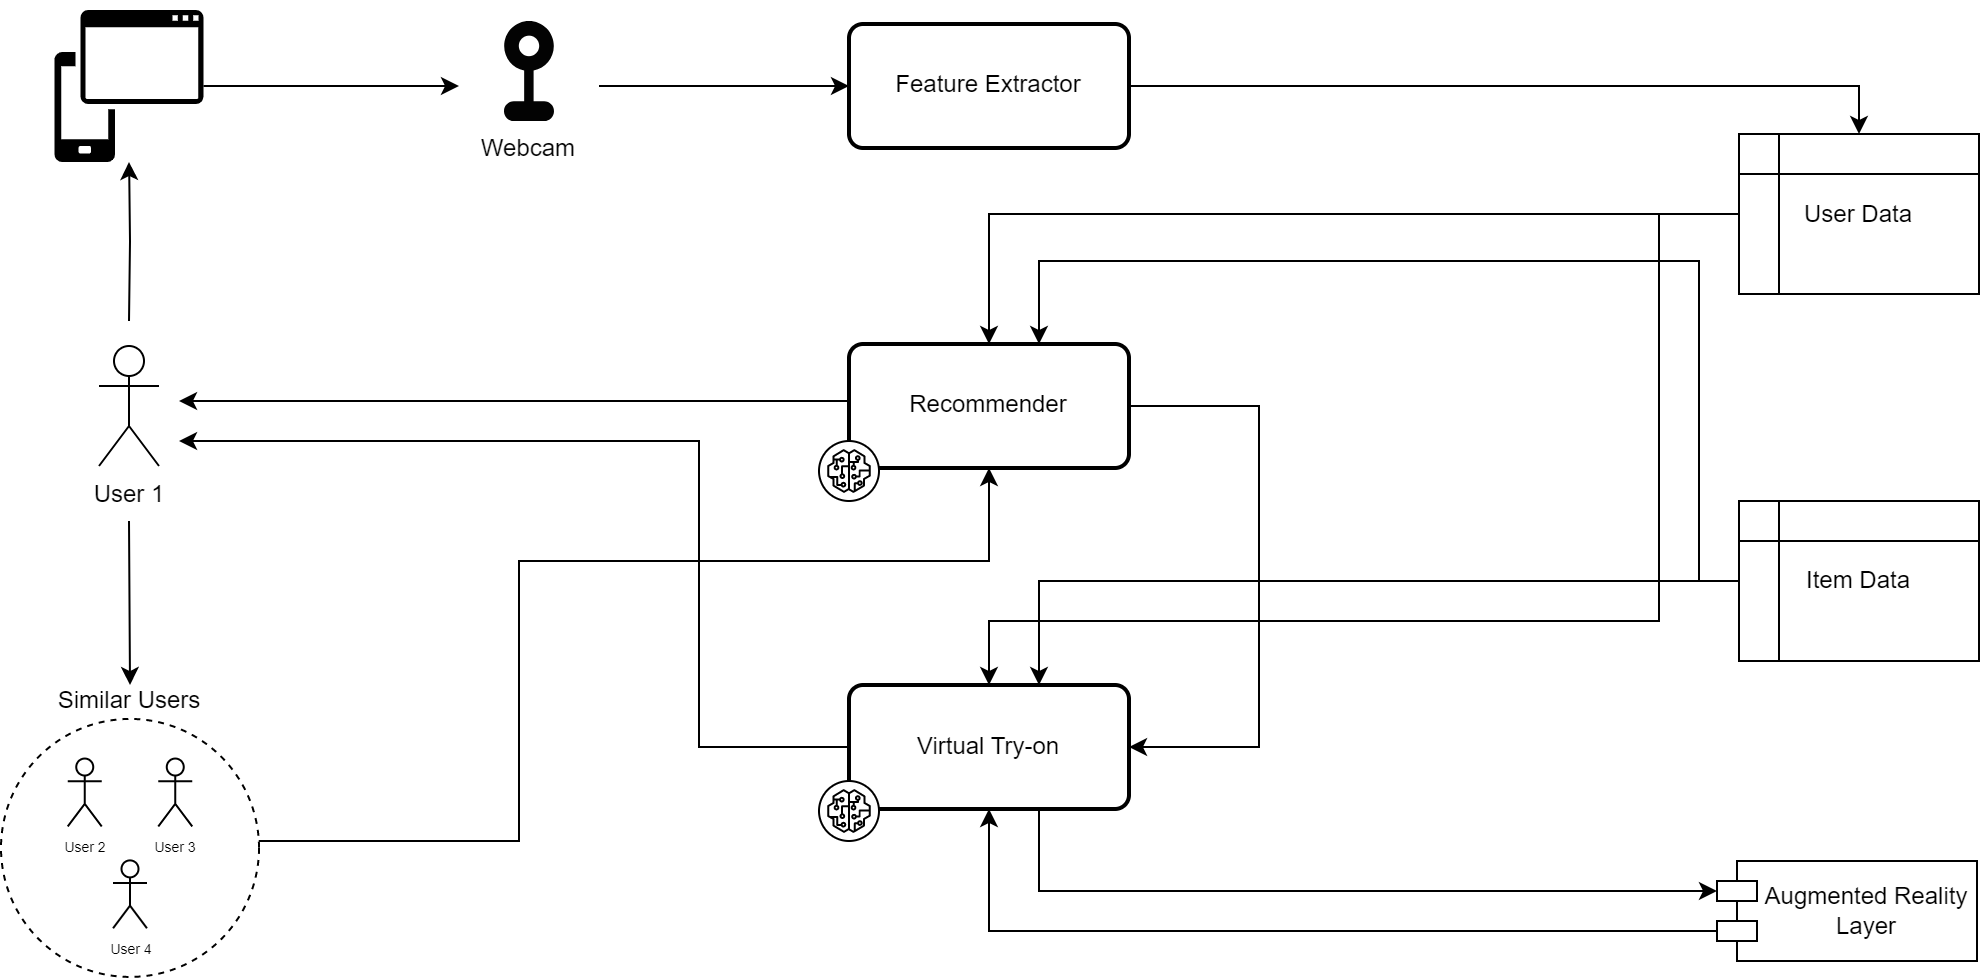
\includegraphics[width=1\textwidth]{components/images/sys-arch.png}
        \caption{System Architecture}
        \label{fig:arch}
    \end{figure}
    We introduce AIRVTON (AI-based Recommendation and Virtual Try-On), an innovative model designed to integrate both recommendation and virtual try-on functionalities within the fashion ecommerce domain. AIRVTON leverages advanced artificial intelligence techniques to provide personalized clothing recommendations while also offering users the ability to virtually try on recommended items.

	The proposed method begins with a comprehensive analysis of historical user data, including past purchases, browsing behavior, and interactions with recommended items. This data is utilized to train machine learning algorithms to understand individual preferences and predict future clothing choices accurately.

	For the recommendation aspect, AIRVTON employs a content-based filtering approach, wherein item attributes and user profiles are utilized to generate personalized recommendations. The model analyzes the visual features of clothing items, such as color, style, and pattern, to identify similarities with previously preferred items and recommend relevant products accordingly.

	Simultaneously, AIRVTON incorporates a sophisticated virtual try-on system, which seamlessly integrates with the recommendation engine. When a user expresses interest in a recommended item, they are provided with the option to virtually try it on. The virtual try-on process involves accurately overlaying the selected clothing item onto the user's image, preserving their pose, body shape, and identity while ensuring natural deformation and realistic rendering of the garment.

	To accomplish this, AIRVTON employs state-of-the-art image synthesis techniques, trained on a diverse dataset of clothing images and human poses. The model dynamically adjusts the appearance of the selected clothing item to fit the user's body proportions and pose, thereby providing an immersive and realistic try-on experience.

\subsection{Fashion Recommendation}
    \begin{figure}[h!]
        \centering
        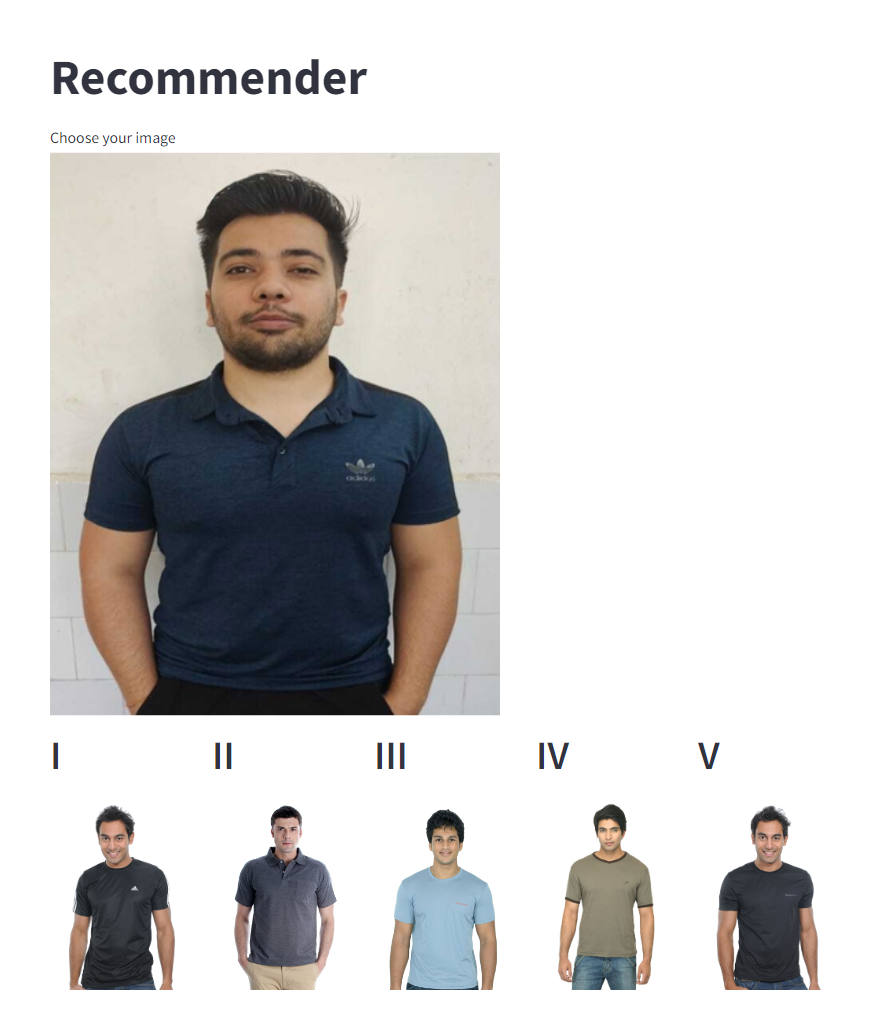
\includegraphics[width=1\textwidth]{components/images/recommender.png}
        \caption{Recommendation System}
        \label{fig:recomm}
    \end{figure}

    In this section, we elaborate on the recommendation aspect of our model AIRVTON, which seamlessly combines Convolutional Neural Network (CNN) architecture with a Nearest Neighbor-based recommender system. This hybrid approach leverages the strengths of both deep learning and traditional recommendation techniques to provide personalized clothing recommendations tailored to individual preferences. We provide a detailed overview of the recommendation pipeline, including the training of neural networks, inventory selection for recommendation generation, and database creation containing item information.

    \subsubsection{Neural Network Training}

    The recommendation pipeline begins with the training of Convolutional Neural Networks (CNNs) on a large dataset of fashion images. These networks are trained using transfer learning techniques, where pre-trained models such as ResNet50 are fine-tuned on the specific task of fashion recommendation. During training, the CNNs learn to extract high-level features from the input images, capturing essential visual characteristics of different clothing items. Additional layers are added to the pre-trained architectures to adapt them to the recommendation task, enabling them to generate embeddings that encode the unique features of each fashion item.

    \subsubsection{Inventory Selection}

    Following neural network training, an inventory is selected for recommendation generation. This inventory comprises a diverse collection of clothing items representing various styles, brands, and categories. Careful selection of the inventory ensures that it adequately covers the preferences and tastes of the target user demographic. The inventory may be curated manually based on expert knowledge or automatically generated using data-driven approaches such as clustering or collaborative filtering.

    \subsubsection{Database Creation}

    Once the inventory is finalized, a corresponding database is created containing detailed information about each item. This information may include attributes such as item name, description, brand, price, and image embeddings generated by the trained neural networks. The database serves as a repository of item information that facilitates efficient and accurate recommendation generation. It allows for fast retrieval of relevant items based on user preferences and provides a comprehensive overview of the available inventory.

    By combining deep learning techniques with traditional recommendation methods, AIRVTON offers a powerful and versatile approach to clothing recommendation. The integration of CNNs enables the model to learn rich representations of fashion items, while the Nearest Neighbor-based recommender leverages these embeddings to provide personalized recommendations. This hybrid approach ensures that AIRVTON can effectively capture the diverse preferences and tastes of users, leading to more accurate and relevant clothing suggestions.

    \subsection{Approach to recommendation system}

	\subsubsection{Recommendation Generation}

    The recommendation process in AIRVTON commences with the utilization of the Nearest Neighbor algorithm, a fundamental technique in recommendation systems, to identify the most relevant products based on the input image. This algorithm compares the features extracted from the input image with those of items in the database, selecting the items that are most similar in terms of visual appearance. By leveraging this approach, AIRVTON generates personalized recommendations that closely align with the user's preferences and style preferences.

    \subsubsection{Neural Network Training}

    Following recommendation generation, the neural networks undergo extensive training to refine their ability to extract meaningful features from fashion images. This training process is crucial for enhancing the model's capacity to understand and interpret the visual characteristics of different clothing items. To achieve this, transfer learning techniques are employed, leveraging pre-trained models such as ResNet50 as a starting point. By initializing the networks with weights learned from large-scale image datasets, the model can effectively capture generic visual features before fine-tuning them to the specific task of fashion recommendation.

    \subsubsection{Fine-tuning with Additional Layers}

    During training, additional layers are incorporated into the final layers of the neural networks, replacing the architecture and weights inherited from ResNet50. This fine-tuning process allows the model to adapt its learned representations to better suit the requirements of the recommendation task at hand. By introducing additional layers, AIRVTON refines its understanding of fashion images, enabling it to capture more nuanced features and nuances that are relevant for generating accurate recommendations. This iterative refinement process ensures that the model can effectively leverage the learned representations to provide personalized and contextually relevant clothing suggestions to users.

    By integrating the Nearest Neighbor algorithm with deep learning techniques such as transfer learning and fine-tuning, AIRVTON offers a robust and versatile approach to clothing recommendation. The combination of these techniques enables the model to leverage both the power of data-driven algorithms and the flexibility of deep learning models, resulting in more accurate, relevant, and personalized recommendations for users.


	To facilitate recommendation generation, our proposed approach employs Sklearn's Nearest Neighbors method, a versatile and efficient algorithm for finding the nearest neighbors of a given data point. This method enables the identification of the nearest neighbors for a given input image, utilizing the Cosine Similarity measure as the similarity metric. The Cosine Similarity measure calculates the cosine of the angle between two vectors, providing a robust measure of similarity that is invariant to the magnitude of the vectors.

    Subsequently, once the nearest neighbors have been identified, the top 5 recommendations are extracted from the database. These recommendations represent the clothing items that are most similar to the input image in terms of visual characteristics such as style, color, and pattern. By selecting the top 5 recommendations, we ensure that a diverse range of options is presented to the user, allowing for greater flexibility and choice in the shopping experience.

    Furthermore, the integration of Convolutional Neural Network (CNN) with the Nearest Neighbor-based recommender enhances the recommendation process in AIRVTON. The CNN leverages deep learning techniques to extract rich and informative features from the input images, capturing subtle nuances and details that may not be captured by traditional recommendation methods alone. These features are then used to generate embeddings that encode the visual characteristics of each clothing item, enabling more accurate and contextually relevant recommendations.

    By combining the power of deep learning with the efficiency of nearest neighbor methods, AIRVTON delivers personalized and contextually relevant recommendations, enhancing the overall shopping experience for users. This hybrid approach ensures that users receive recommendations that are not only visually appealing but also aligned with their individual preferences and tastes, ultimately leading to increased user satisfaction and engagement in the fashion ecommerce domain.

    
    \subsection{Virtual Try-On}
    Given a reference image \( I \in \mathbb{R}^{3 \times H \times W} \) of a person and a clothing image \( c \in \mathbb{R}^{3 \times H \times W} \) (where \( H \) and \( W \) denote the image height and width, respectively), our objective is to synthesize an image \( \hat{I} \in \mathbb{R}^{3 \times H \times W} \) of the person wearing the clothing image \( c \), while preserving the pose and body shape of \( I \).

    To achieve this, we employ the Attire simulation engine and Garment overlay generator components of AIRVTON. Following the training procedure outlined in VITON, we train the model to reconstruct the reference image \( I \) from a clothing-agnostic person representation and the clothing image \( c \) that the person is already wearing. The clothing-agnostic person representation serves to remove any clothing information from \( I \), enabling the model to generalize at test time when presented with arbitrary clothing images.

    Our framework comprises two primary stages: the Attire simulation engine and the Garment overlay generator. Given the clothing-agnostic person representation and the clothing image \( c \), our Attire simulation engine effectively generates the try-on conditions by deforming \( c \) and producing the segmentation map simultaneously. Notably, this generator ensures the absence of misalignment or pixel-squeezing artifacts, maintaining the integrity of the synthesized image.

    Subsequently, the Garment overlay generator synthesizes the final try-on result utilizing the outputs generated by the Attire simulation engine. During testing, we incorporate a discriminator rejection mechanism to filter out incorrect segmentation map predictions, enhancing the overall accuracy and reliability of the virtual try-on process within AIRVTON.

    In the initial pre-processing stage, our approach entails the acquisition of crucial data elements to facilitate subsequent operations. This includes obtaining a segmentation map \( S \in L^{H \times W} \) delineating the person, a clothing mask \( c_m \in L^{H \times W} \), and a pose map \( P \in \mathbb{R}^{3 \times H \times W} \) through the utilization of pre-existing models. Here, \( L \) denotes a set of integers representing semantic labels.

    For the pose map \( P \), we leverage dense pose techniques, which enable the mapping of all pixels within the person regions in the RGB image onto the 3D surface of the individual's body. This step is crucial for preserving the spatial relationships and nuances of the person's pose within the synthesized imagery.

    In order to establish a clothing-agnostic representation of the person, we introduce a clothing-agnostic person image \( I_a \) and a corresponding clothing-agnostic segmentation map \( S_a \), drawing inspiration from the methodology employed in VITON-HD. These elements collectively form the foundation for subsequent stages in our virtual try-on process within AIRVTON.

    In the initial pre-processing stage, our approach entails the acquisition of crucial data elements to facilitate subsequent operations. This includes obtaining a segmentation map \( S \in L^{H \times W} \) delineating the person, a clothing mask \( c_m \in L^{H \times W} \), and a pose map \( P \in \mathbb{R}^{3 \times H \times W} \) through the utilization of pre-existing models. Here, \( L \) denotes a set of integers representing semantic labels.

    For the pose map \( P \), we leverage dense pose techniques, which enable the mapping of all pixels within the person regions in the RGB image onto the 3D surface of the individual's body. This step is crucial for preserving the spatial relationships and nuances of the person's pose within the synthesized imagery.

    In order to establish a clothing-agnostic representation of the person, we introduce a clothing-agnostic person image \( I_a \) and a corresponding clothing-agnostic segmentation map \( S_a \), drawing inspiration from the methodology employed in VITON-HD. These elements collectively form the foundation for subsequent stages in our virtual try-on process within AIRVTON.
    \begin{figure}
        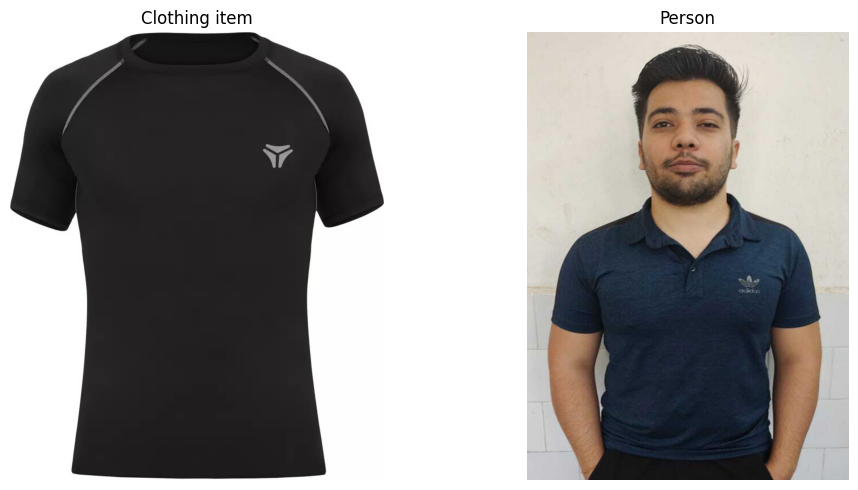
\includegraphics[width=\textwidth]{components/images/output1.png}
        \caption{User Selection}
        \label{fig:user-selection}
    \end{figure}
    \begin{figure}
        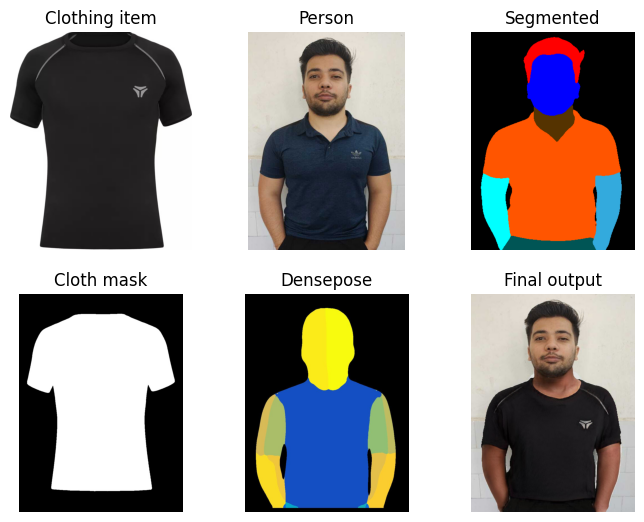
\includegraphics[width=\textwidth]{components/images/output2.png}
        \caption{Outfit Generation}
        \label{fig:outfit-generation}
    \end{figure}

\subsubsection{Attire Simulation Engine}
    In this pivotal stage, our primary objective is to generate the segmentation map \( \hat{S} \) depicting the person adorned with the target clothing item \( c \), while simultaneously deforming \( c \) to conform to the contours of the person's body. The resulting warped clothing image \( \hat{I}_c \) and the synthesized segmentation map \( \hat{S} \) serve as crucial conditions for the subsequent try-on image generation process.

    The overarching architecture of our condition generation process is illustrating the intricate interplay between various components within our try-on condition generator. This generator is comprised of two distinct encoders: a clothing encoder \( E_c \) and a segmentation encoder \( E_s \), along with a decoder.

    Given the input pairs \( (c, c_m) \) and \( (S_a, P) \), our methodology commences by extracting feature pyramids \( \{E_c^k\}_{k=0}^4 \) and \( \{E_s^l\}_{l=0}^4 \) from each encoder, respectively. These extracted features are subsequently fed into the feature fusion blocks of the decoder, where they undergo fusion to predict both the segmentation map and the appearance flow required for warping the clothing image.

    Through careful alignment of conditions, facilitated by the outputs of the last feature fusion block, we derive the warped clothing image \( \hat{I}_c \), the synthesized segmentation map \( \hat{S}_c \), and the resultant segmentation map \( \hat{S} \). This meticulous process ensures the seamless integration of the target clothing item onto the person's body, laying the groundwork for the subsequent stages of virtual try-on within AIRVTON.

\subsubsection{Garment Overlay Generator}
    In this pivotal stage, we synthesize the final try-on image \( \hat{I} \) by seamlessly blending the clothing-agnostic image \( I_a \), the warped clothing image \( \hat{I}_c \), and the pose map \( P \), under the guidance of the synthesized segmentation map \( \hat{S} \). This process forms the crux of our garment overlay generator, which is meticulously designed to ensure the creation of visually appealing and realistic try-on results.

    The garment overlay generator architecture is characterized by a series of residual blocks, complemented by upsampling layers to enhance spatial resolution. Notably, the residual blocks incorporate SPADE as normalization layers, with modulation parameters inferred from \( \hat{S} \). Additionally, the input \( (I_a, \hat{I}_c, P) \) undergoes resizing and concatenation with the activation before each residual block, facilitating effective information flow and feature integration.

    During training, the generator is subjected to the same loss functions utilized in SPADE and pix2pixHD, ensuring consistency and coherence with established methodologies in image synthesis. Comprehensive details regarding the model architecture, hyperparameters, and objective function formulations are provided in the supplementary material, offering insights into the intricacies of our approach within AIRVTON.

\section{Evaluation Metrics}

In order to assess the performance of our proposed model, AIRVTON, we utilized two key evaluation metrics: Structural Similarity Index (SSIM) and Fréchet Inception Distance (FID). These metrics provide valuable insights into the quality and fidelity of the generated images compared to ground truth or reference images.

\subsection{Structural Similarity Index (SSIM)}

The Structural Similarity Index (SSIM) is a widely used metric for measuring the similarity between two images. It takes into account luminance, contrast, and structure, providing a comprehensive measure of image similarity. SSIM values range from -1 to 1, with 1 indicating perfect similarity and -1 indicating complete dissimilarity.

Mathematically, the SSIM between two images \(I\) and \(I'\) is computed as:

\[
\text{SSIM}(I, I') = \frac{{2 \mu_I \mu_{I'} + C_1}}{{\mu_I^2 + \mu_{I'}^2 + C_1}} \times \frac{{2 \sigma_{I,I'} + C_2}}{{\sigma_I^2 + \sigma_{I'}^2 + C_2}}
\]

where:
\begin{itemize}
  \item \(\mu_I\) and \(\mu_{I'}\) are the mean intensities of \(I\) and \(I'\) respectively.
  \item \(\sigma_I\) and \(\sigma_{I'}\) are the standard deviations of \(I\) and \(I'\) respectively.
  \item \(\sigma_{I,I'}\) is the covariance between \(I\) and \(I'\).
  \item \(C_1\) and \(C_2\) are constants to stabilize the division with weak denominator.
\end{itemize}

A higher SSIM score indicates greater similarity between the generated images and the ground truth, with a perfect score of 1 indicating identical images.

\subsection{Fréchet Inception Distance (FID)}

The Fréchet Inception Distance (FID) is a measure of the similarity between two datasets of images. It computes the distance between the feature representations of real and generated images, using an Inception-v3 model pretrained on a large dataset.

Mathematically, the FID between two datasets \(X\) and \(Y\) is computed as:

\[
\text{FID}(X, Y) = \| \mu_X - \mu_Y \|^2 + \text{Tr}(C_X + C_Y - 2(C_XC_Y)^{1/2})
\]

where:
\begin{itemize}
  \item \(\mu_X\) and \(\mu_Y\) are the mean feature vectors of the real and generated images, respectively.
  \item \(C_X\) and \(C_Y\) are the covariance matrices of the feature vectors of the real and generated images, respectively.
\end{itemize}

A lower FID score indicates better similarity between the distributions of real and generated images, with a perfect score of 0 indicating identical distributions.

These evaluation metrics provide valuable quantitative insights into the performance of our model, allowing us to assess its effectiveness in generating realistic and high-quality fashion images.

\section{Results}

In this section, we present the results of our experiments conducted to evaluate the performance of AIRVTON, our proposed model for fashion recommendation and virtual try-on. We employ two key evaluation metrics, namely Structural Similarity Index (SSIM) and Fréchet Inception Distance (FID), to assess the quality and fidelity of the generated try-on images produced by AIRVTON. Through rigorous experimentation and analysis, we aim to demonstrate the effectiveness of AIRVTON in generating realistic and visually appealing try-on results that closely resemble the ground truth images from the dataset. The following subsections provide detailed insights into the SSIM and FID evaluation results, shedding light on the performance and capabilities of AIRVTON in the context of fashion ecommerce and virtual fitting solutions.


\begin{table}[htbp]
    \caption{Evaluation Results}
    \label{tab:evaluation_results}
    \centering
    \begin{tabular}[htbp]{|l|l|l|l|l|l|l|}
    \hline
        ~ &  \multicolumn{2}{c|}{\textbf{192$\times$256}} &  \multicolumn{2}{c|}{\textbf{384$\times$512}} & \multicolumn{2}{c|}{\textbf{768$\times$1024}} \\ 
        ~ &  SSIM ${\uparrow}$ &  FID ${\downarrow}$ &  SSIM ${\uparrow}$  &  FID ${\downarrow}$ &  SSIM ${\uparrow}$ &  FID ${\downarrow}$ \\ \hline
        CP-VTON &  0.748  &  30.07  &  0.723  &  30.30  &  0.728  &  43.19  \\ 
        ACGPN &  0.772  &  11.25  &  0.935  &  14.41  &  0.845  &  43.24  \\ 
        VITON-HD &  0.816  &  16.32  &  0.751  &  11.61  &  0.813  &  11.63  \\ 
        PF-AFN &  -    &  -    &  -    &  -    &  -    &  13.99  \\ 
        HR-VITON &  0.888  &  9.39  &  0.825  &  9.88  &  0.895  &  10.83  \\ 
        \textbf{AIRVTON (Ours)} &  \textbf{0.818}  &  \textbf{9.60}  &  \textbf{0.802}  &  \textbf{10.18}  &  \textbf{0.976}  &  \textbf{10.67}  \\ \hline
    \end{tabular}
\end{table}

\subsection{SSIM Evaluation}

We evaluated the structural similarity index (SSIM) between the generated try-on images produced by AIRVTON and the ground truth images from the dataset. The SSIM scores were computed across a sample of 1000 images randomly selected from the test set. Table~\ref{tab:ssim_results} presents the mean SSIM scores along with the standard deviation.


\begin{table}[htbp]
  \caption{SSIM Evaluation Results}
  \label{tab:ssim_results}
  \centering
  \begin{tabular}{lcc}
    \toprule
    \textbf{Model} & \textbf{Mean SSIM} & \textbf{Standard Deviation} \\
    \midrule
    AIRVTON & 0.976 & 0.03 \\
    \bottomrule
  \end{tabular}
\end{table}

The results indicate that AIRVTON achieved a mean SSIM score of 0.976 with a standard deviation of 0.03, showcasing a high level of structural similarity between the generated try-on images and the ground truth images.

\subsection{FID Evaluation}

For the Fréchet Inception Distance (FID) evaluation, we compared the feature distributions of the generated try-on images and the ground truth images using an Inception-v3 model pretrained on a large dataset. Table~\ref{tab:fid_results} summarizes the FID scores obtained from this evaluation.

\begin{table}[htbp]
  \caption{FID Evaluation Results}
  \label{tab:fid_results}
  \centering
  \begin{tabular}{lc}
    \toprule
    \textbf{Model} & \textbf{FID Score} \\
    \midrule
    AIRVTON & 10.67 \\
    \bottomrule
  \end{tabular}
\end{table}

The FID score obtained for AIRVTON is 10.67, indicating a relatively low distance between the feature distributions of the generated try-on images and the ground truth images. This suggests that AIRVTON effectively captures the underlying structure and characteristics of the fashion items, producing results that closely resemble the ground truth images.

The results of both SSIM and FID evaluations demonstrate the effectiveness of AIRVTON in generating realistic and high-quality try-on images, showcasing its potential for enhancing the online shopping experience in the fashion ecommerce domain.

\section{Testing}

In this section, we outline the test cases conducted to validate the functionality and robustness of AIRVTON. The following test cases cover key aspects of the system, ensuring its reliability and performance in different scenarios.

\subsection{test\_save\_file}
\begin{itemize}
  \item \textbf{Description}: This test case verifies the functionality of the save file feature in AIRVTON.
  \item \textbf{Steps}:
    \begin{enumerate}
      \item Upload a sample image to AIRVTON.
      \item Click on the "Save" button to save the image.
    \end{enumerate}
  \item \textbf{Expected Outcome}: The uploaded image should be saved successfully to the specified location.
\end{itemize}

\subsection{test\_save\_empty\_file}
\begin{itemize}
  \item \textbf{Description}: This test case validates the behavior of AIRVTON when attempting to save an empty file.
  \item \textbf{Steps}:
    \begin{enumerate}
      \item Attempt to save an empty file using AIRVTON.
    \end{enumerate}
  \item \textbf{Expected Outcome}: AIRVTON should display an error message indicating that the file cannot be saved as it is empty.
\end{itemize}

\subsection{test\_no\_uploaded\_file}
\begin{itemize}
  \item \textbf{Description}: This test case examines the response of AIRVTON when no file is uploaded.
  \item \textbf{Steps}:
    \begin{enumerate}
      \item Access AIRVTON without uploading any file.
    \end{enumerate}
  \item \textbf{Expected Outcome}: AIRVTON should display a message prompting the user to upload a file.
\end{itemize}

\subsection{test\_streamlit\_app\_title}
\begin{itemize}
  \item \textbf{Description}: This test case verifies the title of the Streamlit web application.
  \item \textbf{Steps}:
    \begin{enumerate}
      \item Access AIRVTON web application.
    \end{enumerate}
  \item \textbf{Expected Outcome}: The title of the web application should be "AIRVTON - Fashion Recommendation and Virtual Try-On".
\end{itemize}

\subsection{test\_save\_file\_path}
\begin{itemize}
  \item \textbf{Description}: This test case checks if the file is saved at the specified path.
  \item \textbf{Steps}:
    \begin{enumerate}
      \item Upload a sample image to AIRVTON.
      \item Click on the "Save" button to save the image.
    \end{enumerate}
  \item \textbf{Expected Outcome}: The uploaded image should be saved at the specified file path on the local system.
\end{itemize}
\begin{figure}
    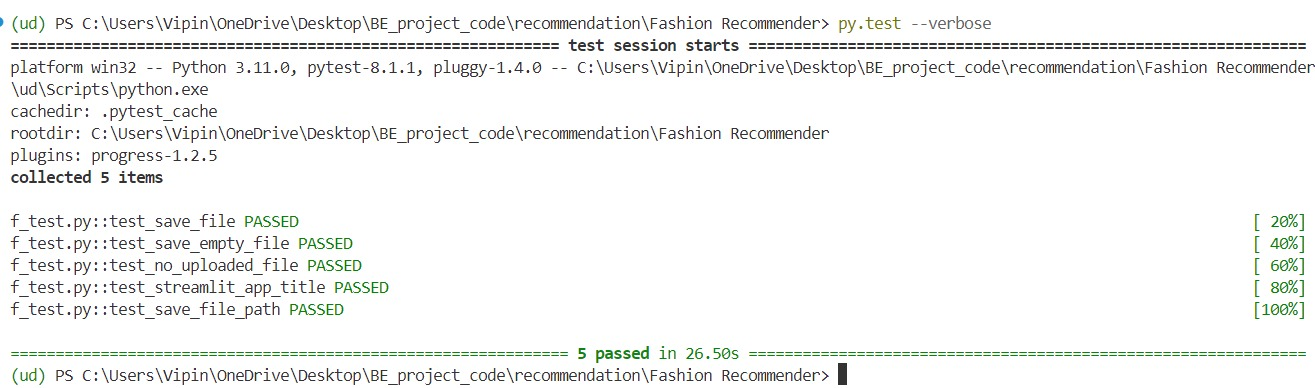
\includegraphics[width=\textwidth]{components/images/test_case.jpg}
    \caption{Test Case Snapshot}
    \label{fig:test-case}
\end{figure}
